% Полезные ссылки:
% * https://habrahabr.ru/post/144648/ - Диплом бакалавра в LaTeX, или ДСТУ 3008-95 в 150 строк
% * http://dkhramov.dp.ua/Comp/NIRReportDSTU300895 - Оформление отчета о НИР в LaTeX
% * http://dkhramov.dp.ua/index.php?n=Comp.CyrillicInListingsTex - Оформление исходного кода в документах LaTeX
% * http://mydebianblog.blogspot.ru/2012/12/latex.html - Как оформить исходный код программ в LaTeX без адских страданий
% * http://aakinshin.blogspot.ru/2014/01/latex-minted.html -  minted: Оформляем исходный код в LaTeX
% * http://s.arboreus.com/2008/12/russian-thesis-in-latex.html - советы: Диссертация в LaTeX

\documentclass[a4paper,14pt]{article}
%\documentclass[a4paper,12pt]{article}

% Русский язык (LaTeX)
%\usepackage[T1,T2A]{fontenc}
%\usepackage[utf8]{inputenc}
%\usepackage[english,russian]{babel}

% Русский язык и шрифты (XeLaTeX)
\usepackage{xunicode}
\usepackage{xltxtra}
\usepackage[english,russian]{babel}
\usepackage{xecyr}
\defaultfontfeatures{Ligatures={TeX}}
\setsansfont[Path=./fonts/arial/, UprightFont=*, ItalicFont=*i, BoldFont=*bd, BoldItalicFont=*bi]{arial}
\setmonofont[Path=./fonts/courier_new/, UprightFont=*, ItalicFont=*i, BoldFont=*bd, BoldItalicFont=*bi, Mapping=]{cour}
\setmainfont[Path=./fonts/times_new_roman/, UprightFont=*, ItalicFont=*i, BoldFont=*bd, BoldItalicFont=*bi]{times}

% Отступ у первого абзаца
\usepackage[indentfirst]{titlesec}

% Возможность сделать 14-й шрифт
\usepackage{extsizes}
\usepackage{anyfontsize}

% Междустрочный интервал
%\linespread{1.35}
\usepackage[nodisplayskipstretch]{setspace}
%\onehalfspacing
\setstretch{1.4}
% Нет интервала между элементами списков
\usepackage{enumitem}
\setlist{nosep}
% Отступы в списках
%\setitemize[0]{leftmargin=0pt, itemindent=35pt}

% Интервал между абзацами
\setlength{\parskip}{6pt}

% Поля страницы
\usepackage[left=3cm,top=2cm,right=1cm,bottom=2cm]{geometry}

% Отступ для абзаца
\setlength{\parindent}{1cm}

% Литература с точки + нормальные ссылки
\usepackage[square,numbers,sort&compress]{natbib}
\renewcommand{\bibnumfmt}[1]{#1.\hfill}
%\def\@biblabel#1{#1.}

% Начать нумерацию страниц не с 1
%\setcounter{page}{4}

% Картинки
\usepackage{graphicx}

% Каталог для картинок
\graphicspath{ {./images/} }

% Разные таблицы
\usepackage{tabularx, multirow}
\newcolumntype{L}[1]{>{\hsize=#1\hsize\raggedright\arraybackslash}X}
\newcolumntype{R}[1]{>{\hsize=#1\hsize\raggedleft\arraybackslash}X}
\newcolumntype{C}[1]{>{\hsize=#1\hsize\centering\arraybackslash}X}
%\newcolumntype{C}[2]{>{\hsize=#1\hsize\columncolor{#2}\centering\arraybackslash}X}

% Таблицы и рисунки по ГОСТу
\usepackage[tableposition=top, singlelinecheck=false]{caption}
\DeclareCaptionLabelFormat{gostfigure}{Рисунок #2}\DeclareCaptionLabelFormat{gosttable}{Таблица #2}
\DeclareCaptionLabelSeparator{gost}{~---~}
\captionsetup{labelsep=gost}
\captionsetup*[figure]{labelformat=gostfigure, justification=centering}
\captionsetup*[table]{labelformat=gosttable, justification=raggedright}
\usepackage{subfig}
\renewcommand{\thesubfigure}{\asbuk{subfigure}}
% в рисунках: h - "хотелось бы картинку здесь"; h! - "очень хочу картинку здесь"; H - "ХОЧУ картинку здесь и баста", p - на отдельной странице, t - сверху
% Управление плавающими штуковинами (рисунками, таблицами, etc)
\usepackage{float}

% Точки после номеров разделов
\usepackage[subfigure]{tocloft}
\renewcommand{\cftsecaftersnum}{.}
\renewcommand{\cftsubsecaftersnum}{.}
\makeatletter
\def\@seccntformat#1{\csname the#1\endcsname.\ }
\makeatother

% Даешь подсекции в оглавление
\setcounter{tocdepth}{3}

% Размер шрифтов в названиях секций/подсекций
\addto{\captionsrussian}{\renewcommand*{\contentsname}{{\fontsize{14}{16}\selectfont Содержание}}}
\titleformat{\section}{\normalfont\fontsize{14}{16}\bfseries}{\thesection.}{1ex}{}
\titleformat{\subsection}{\normalfont\fontsize{14}{16}\bfseries\itshape}{\thesubsection.}{1ex}{}
\titleformat{\subsubsection}{\normalfont\fontsize{14}{16}\bfseries\itshape}{\thesubsubsection.}{1ex}{}

% Размер шрифтов в содержании
\renewcommand\cftsecfont{\normalfont}
\renewcommand\cftsecpagefont{\normalfont}

% Точки в секциях
% https://tex.stackexchange.com/questions/53898/how-to-get-lines-with-dots-in-the-table-of-contents-for-sections
\renewcommand{\cftsecleader}{\cftdotfill{\cftdotsep}}

% Запрет висячих строк
\clubpenalty=10000
\widowpenalty=10000

% Для формул
\usepackage{amsmath}
\usepackage{mathtools}
\usepackage{amsfonts}
\usepackage{amssymb}
\usepackage{amsbsy}

% Работа с цветом
% http://habrahabr.ru/post/52166/
\usepackage[usenames]{color}
\usepackage{colortbl}

% Разные подчеркивания
% https://tex.stackexchange.com/questions/27258/how-do-i-write-underline-text-but-with-a-dotted-line
\usepackage{tikz}
\newcommand{\dotunderline}[1]{%
    \tikz[baseline=(todotted.base)]{
        \node[inner sep=1pt,outer sep=0pt] (todotted) {#1};
        \draw[densely dotted] (todotted.south west) -- (todotted.south east);
    }%
}%

% Раскопировать пробелы
\newcommand\spacedfill[1]{\makebox[#1]{\leaders\hbox{~}\hfill}}

% Код программы
% http://mydebianblog.blogspot.ru/2012/12/latex.html
\usepackage{verbatim}

% Структурированный pdf
\usepackage[bookmarksnumbered=true,bookmarksopen=true,breaklinks=true,pdfborder={0 0 0},linktoc=all]{hyperref}

% Минимальное количество букв, которые можно переносить
\righthyphenmin=2

% Борьба с overfull
\tolerance=300000

% Перенос знаков во внутритекстовых формулах (использовать так $a\hm+b\hm+c\hm+d$)
%\newcommand*{\hm}[1]{#1\nobreak\discretionary{}{\hbox{$\mathsurround=0pt #1$}}{}}
% Можно также просто запретить переносить знаки операций и отношений
\binoppenalty=10000
\relpenalty=10000

%
\title{Отчет по производственной практике}
\author{Жигалов П.С.}

% Счетчики страниц и всякого разного
\usepackage{lastpage, totcount}
% Счетчик рисунков
\newtotcounter{foofigure}
\makeatletter
\renewenvironment{figure}[1][\fps@figure]{
  \edef\@tempa{\noexpand\@float{figure}[#1]}
  \@tempa
  \addtocounter{foofigure}{1}
}{
  \end@float
}
\makeatother
% Счетчик таблиц
\newtotcounter{footable}
\makeatletter
\renewenvironment{table}[1][\fps@table]{
  \edef\@tempa{\noexpand\@float{table}[#1]}
  \@tempa
  \addtocounter{footable}{1}
}{
  \end@float
}
\makeatother
% Счетчик источников в списке литературы
\newtotcounter{foobibitem}
\def\oldbibitem{}
\let\oldbibitem=\bibitem
\def\bibitem{\stepcounter{foobibitem}\oldbibitem}

% Команды и сокращения
\renewcommand{\Re}{\mathop{\mathrm{Re}}\nolimits}
\renewcommand{\Im}{\mathop{\mathrm{Im}}\nolimits}
\newcommand{\Jmp}[1]{[\![ { #1 } ]\!]}
\newcommand{\Avg}[1]{\{\!\!\{ { #1 } \}\!\!\}}
\newcommand{\Flux}[1]{\reallywidehat{ #1 } }
\newcommand{\CalTau}{\mathcal{T}}
\newcommand{\CalEps}{\mathcal{E}}
\newcommand{\CalF}{\mathcal{F}}

% =============================================================================

\begin{document}

\begin{titlepage}
	\begin{spacing}{0.75}
		\begin{center}
			{~}\\ 
			\vspace{-0.55cm}
			{\fontsize{12}{14}\selectfont \MakeUppercase{Министерство образования и науки Российской Федерации}}\\
			\vspace{0.4cm}
			{\fontsize{11}{14}\selectfont ФЕДЕРАЛЬНОЕ ГОСУДАРСТВЕННОЕ БЮДЖЕТНОЕ ОБРАЗОВАТЕЛЬНОЕ УЧРЕЖДЕНИЕ}\\
			{\fontsize{11}{14}\selectfont ВЫСШЕГО ОБРАЗОВАНИЯ}\\
			\vspace{0.48cm}
			{\fontsize{12}{14}\selectfont <<\MakeUppercase{Новосибирский государственный технический университет}>>}\\
			\vspace{-0.25cm}
			\noindent\rule{16cm}{0.7pt}
			{~}\\
			\vspace{0.8cm}
			{\fontsize{12}{14}\selectfont Кафедра \dotunderline{\spacedfill{4cm}{\fontsize{14}{14}\selectfont Вычислительных технологий}\spacedfill{4cm}}}\\
			\vspace{-0.15cm}
			{\fontsize{8}{14}\selectfont \spacedfill{1.8cm}(полное название кафедры)}\\
			\vspace{1.9cm}
			{\fontsize{12}{14}\selectfont \dotunderline{\spacedfill{1.5cm}{\fontsize{14}{14}\selectfont Петр Сергеевич Жигалов}\spacedfill{1.5cm}}}\\
			{\fontsize{8}{14}\selectfont (И. О. Фамилия студента – автора работы)}\\
			\vspace{0.8cm}
			{\fontsize{12}{14}\selectfont \dotunderline{\spacedfill{0.9cm}{\fontsize{14}{14}\selectfont Анализ систем источник-приемник в задачах морской геоэлектрики}\spacedfill{0.9cm}}}\\
			{\fontsize{8}{14}\selectfont (полное название темы магистерской диссертации)}\\
			{\fontsize{12}{14}\selectfont \dotunderline{\spacedfill{16cm}}}\\
			{\fontsize{8}{14}\selectfont ~}\\
			{\fontsize{12}{14}\selectfont \dotunderline{\spacedfill{16cm}}}\\
			\vspace{1.1cm}
			{\fontsize{12}{14}\selectfont \textbf{МАГИСТЕРСКАЯ ДИССЕРТАЦИЯ}}\\
			{\fontsize{12}{14}\selectfont по направлению высшего образования}\\
			\vspace{0.4cm}
			{\fontsize{12}{14}\selectfont \dotunderline{\spacedfill{1.75cm}{\fontsize{14}{14}\selectfont 01.04.02 – Прикладная математика и информатика}\spacedfill{3.75cm}}}\\
			{\fontsize{8}{14}\selectfont (код и наименование направления подготовки магистра)}\\
			\vspace{0.2cm}
			{\fontsize{12}{14}\selectfont \dotunderline{\spacedfill{16cm}}}\\
			\vspace{0.35cm}
			{\fontsize{12}{14}\selectfont \dotunderline{\spacedfill{1.7cm}{\fontsize{14}{14}\selectfont факультет прикладной математики и информатики}\spacedfill{3.7cm}}}\\
			{\fontsize{8}{14}\selectfont (факультет)}\\
		\end{center}
		{\fontsize{12}{14}\selectfont Тема диссертации утверждена приказом по НГТУ № 4931/2~~~от~~~<<15>>~~~октября~~~2014 г.}\\
		\begin{center}
			\hfill
			\parbox[t][4em][t]{0.49\textwidth} {
				\begin{center}
					\vspace{0.1cm}
					{\fontsize{12}{14}\selectfont Руководитель}\\
					\vspace{0.3cm}
					{\fontsize{12}{14}\selectfont \dotunderline{\spacedfill{1.6cm}{\fontsize{14}{14}\selectfont Шурина Э.П.}\spacedfill{1.6cm}}}\\
					\vspace{-0.05cm}
					{\fontsize{8}{14}\selectfont (фамилия, И., О.)}\\
					\vspace{0.2cm}
					{\fontsize{12}{14}\selectfont \dotunderline{\spacedfill{1.25cm}{\fontsize{14}{14}\selectfont д.т.н., профессор}\spacedfill{1.25cm}}}\\
					\vspace{-0.05cm}
					{\fontsize{8}{14}\selectfont (уч. степень, уч. звание)}\\
				\end{center}
			}\\
			\vfill
			{\fontsize{12}{14}\selectfont Новосибирск, 2016 г.}\\
			\vspace{0.9cm}
		\end{center}
	\end{spacing}
\end{titlepage}
\clearpage
\begin{titlepage}
	\begin{spacing}{0.75}
		\begin{center}
			{~}\\ 
			\vspace{0.3cm}
			{\fontsize{12}{14}\selectfont \MakeUppercase{Министерство образования и науки Российской Федерации}}\\
			\vspace{0.4cm}
			{\fontsize{11}{14}\selectfont ФЕДЕРАЛЬНОЕ ГОСУДАРСТВЕННОЕ БЮДЖЕТНОЕ ОБРАЗОВАТЕЛЬНОЕ УЧРЕЖДЕНИЕ}\\
			{\fontsize{11}{14}\selectfont ВЫСШЕГО ОБРАЗОВАНИЯ}\\
			\vspace{0.48cm}
			{\fontsize{12}{14}\selectfont <<\MakeUppercase{Новосибирский государственный технический университет}>>}\\
			\vspace{-0.25cm}
			\noindent\rule{16cm}{0.7pt}
			{~}\\
			\vspace{0.8cm}
			{\fontsize{12}{14}\selectfont Кафедра \dotunderline{\spacedfill{4cm}{\fontsize{14}{14}\selectfont Вычислительных технологий}\spacedfill{4cm}}}\\
			\vspace{-0.15cm}
			{\fontsize{8}{14}\selectfont \spacedfill{1.8cm}(полное название кафедры)}\\
			\vspace{0.2cm}
			\hfill
			\parbox[t][4em][t]{0.42\textwidth} {
				\begin{center}
					\vspace{-0.4cm}
					{\fontsize{12}{14}\selectfont УТВЕРЖДАЮ}\\
					\vspace{0.0cm}
				\end{center}
				\begin{flushright}
					{\fontsize{12}{14}\selectfont Зав. кафедрой ~\dotunderline{\spacedfill{0.5cm}{\fontsize{14}{14}\selectfont Шокин Ю.И.}\spacedfill{0.5cm}}~~~}\\
					\vspace{-0.1cm}
					{\fontsize{8}{14}\selectfont (фамилия, И., О.)\spacedfill{1.3cm}}\\
					\vspace{0.2cm}
					{\fontsize{12}{14}\selectfont \dotunderline{\spacedfill{3.75cm}}~~~}\\
					\vspace{-0.1cm}
					{\fontsize{8}{14}\selectfont (подпись, дата)\spacedfill{1.3cm}}\\
				\end{flushright}
			}\\
			\vspace{2.4cm}
			{\fontsize{12}{14}\selectfont \textbf{ЗАДАНИЕ}}\\
			\vspace{0.04cm}
			{\fontsize{12}{14}\selectfont \textbf{на магистерскую диссертацию}}\\
			\vspace{-0.1cm}
			\begin{flushleft}
				{\spacedfill{0.55cm} \fontsize{12}{14}\selectfont студенту \dotunderline{\spacedfill{4cm}{\fontsize{14}{14}\selectfont Жигалову Петру Сергеевичу}\spacedfill{4.25cm}}}\\
				\vspace{-0.05cm}
				{\spacedfill{7.2cm} \fontsize{8}{14}\selectfont (фамилия, имя, отчество)}\\
				\vspace{0.3cm}
				{\spacedfill{0.55cm} \fontsize{12}{14}\selectfont факультета \dotunderline{\spacedfill{2.5cm}{\fontsize{14}{14}\selectfont прикладной математики и информатики}\spacedfill{2.95cm}}}\\
				\vspace{0.35cm}
				{\spacedfill{0.55cm} \fontsize{12}{14}\selectfont Направление подготовки \dotunderline{\spacedfill{0.4cm}{\fontsize{14}{14}\selectfont 01.04.02 – Прикладная математика и информатика}\spacedfill{0.45cm}}}\\
				\vspace{-0.05cm}
				{\spacedfill{7.5cm} \fontsize{8}{14}\selectfont (код и наименование направления подготовки магистра)}\\
				\vspace{0.1cm}
				{\spacedfill{0.55cm} \dotunderline{\spacedfill{15.95cm}}}\\
				\vspace{0.35cm}
				{\spacedfill{0.55cm} \fontsize{12}{14}\selectfont Магистерская программа \dotunderline{\spacedfill{1.0cm}{\fontsize{14}{14}\selectfont Математическое моделирование} \spacedfill{3.45cm}}}\\
				\vspace{-0.05cm}
				{\spacedfill{9.3cm} \fontsize{8}{14}\selectfont (наименование программы)}\\
				\vspace{0.05cm}
				{\spacedfill{0.55cm} \dotunderline{\spacedfill{2.7cm}{\fontsize{14}{14}\selectfont детерминированных и стохастических процессов} \spacedfill{2.75cm}}}\\
				\vspace{0.35cm}
				{\spacedfill{0.55cm} \fontsize{12}{14}\selectfont Тема \dotunderline{\spacedfill{0.3cm}{\fontsize{14}{14}\selectfont Анализ систем источник-приемник в задачах морской геоэлектрики} \spacedfill{0.3cm}}}\\
				\vspace{-0.05cm}
				{\spacedfill{8.1cm} \fontsize{8}{14}\selectfont (полное название темы)}\\
				\vspace{0.1cm}
				{\spacedfill{0.55cm} \dotunderline{\spacedfill{15.95cm}}}\\
				\vspace{0.4cm}
				{\spacedfill{0.55cm} \fontsize{12}{14}\selectfont Цели работы {\fontsize{14}{14}\selectfont Lorem Ipsum}}\\
				\vspace{-0.35cm}
				{\spacedfill{3.05cm} \dotunderline{\spacedfill{13.45cm}}}\\
				\vspace{0.15cm}
				{\spacedfill{0.55cm} \fontsize{14}{14}\selectfont Lorem Ipsum}\\
				\vspace{-0.35cm}
				{\spacedfill{0.55cm} \dotunderline{\spacedfill{15.95cm}}}\\
				\vspace{0.15cm}
				{\spacedfill{0.55cm} \fontsize{14}{14}\selectfont Lorem Ipsum}\\
				\vspace{-0.35cm}
				{\spacedfill{0.55cm} \dotunderline{\spacedfill{15.95cm}}}\\
				\vspace{0.15cm}
				{\spacedfill{0.55cm} \fontsize{14}{14}\selectfont Lorem Ipsum}\\
				\vspace{-0.35cm}
				{\spacedfill{0.55cm} \dotunderline{\spacedfill{15.95cm}}}\\
				\vspace{0.25cm}
				{\spacedfill{0.55cm} \dotunderline{\spacedfill{15.95cm}}}\\
				\vspace{-0.6cm}
				\parbox[t][4em][t]{0.38\textwidth} {
					\begin{center}
						\vspace{0.1cm}
						{\fontsize{12}{14}\selectfont Руководитель}\\
						\vspace{0.15cm}
						{\fontsize{12}{14}\selectfont \dotunderline{\spacedfill{0.6cm}{\fontsize{14}{14}\selectfont Шурина Э.П.}\spacedfill{0.6cm}}}\\
						\vspace{-0.07cm}
						{\fontsize{8}{14}\selectfont (фамилия, И., О.)}\\
						\vspace{0.05cm}
						{\fontsize{12}{14}\selectfont \dotunderline{\spacedfill{0.25cm}{\fontsize{14}{14}\selectfont д.т.н., профессор}\spacedfill{0.25cm}}}\\
						\vspace{-0.07cm}
						{\fontsize{8}{14}\selectfont (уч. степень, уч. звание)}\\
						\vspace{0.25cm}
						{\fontsize{12}{14}\selectfont \dotunderline{\spacedfill{4.1cm}}}\\
						\vspace{-0.17cm}
						{\fontsize{8}{14}\selectfont (подпись, дата)}\\
					\end{center}
				}\\
			\end{flushleft}
		\end{center}
	\end{spacing}
\end{titlepage}
\setcounter{page}{3}

% =============================================================================

\begin{titlepage}
	\clearpage
	\phantomsection
	\section*{Аннотация}

	Отчет \begin{NoHyper}{\pageref{LastPage}}\end{NoHyper}~с., \total{foofigure}~рис., \total{footable}~табл., \total{foobibitem}~источников, 1~прил.

	СИСТЕМА УРАВНЕНИЙ МАКСВЕЛЛА, УРАВНЕНИЕ ГЕЛЬМГОЛЬЦА, ВЕКТОРНЫЙ МКЭ, ТЕТРАЭДРАЛЬНЫЙ КОНЕЧНЫЙ ЭЛЕМЕНТ, МОРСКАЯ ГЕОЭЛЕКТРИКА, НЕФТЯНЫЕ МЕСТОРОЖДЕНИЯ

	Объектом исследования является поведение электрического поля в недрах земли под слоем морской воды.

	Цель работы – решение трехмерной прямой задачи морской геоэлектрики векторным методом конечных элементов.

	В процессе работы проводилось численное моделирование электрического поля векторным методом конечных элементов, сравнивались результаты на разных частотах и разных комбинациях материалов с различными электрофизическими свойствами.

	В результате исследования было получено представление электрического поля в сложно построенных средах.

\end{titlepage}
\setcounter{page}{4}

% =============================================================================

\tableofcontents

% =============================================================================

\clearpage
\phantomsection
\section*{Введение}
\addcontentsline{toc}{section}{Введение}

% =============================================================================

В современном мире экономика многих стран, таких как Россия, Швеция, Канада, зависит от цены на нефть. Несмотря на то, что цены на углеводороды снижаются, конкуренция за обладание ими не угасает, порой доходя и до вооруженных конфликтов. Таким образом, все более актуальными становятся задачи, связанные с геологоразведкой, особенно в недрах земли, скрытых под толщей морской воды. Это объясняется тем, что, по оценкам специалистов, только на территории Северного Ледовитого океана может находиться до 25 процентов мировых запасов нефти и газа~\citep{shurina, gabrielsen}.

Задачи морской геоэлектрики имеют ряд отличительных особенностей. К ним можно отнести изменение электропроводности морской воды в зависимости от глубины. Это обусловлено различной соленостью и температурой разных слоев морской воды. Кроме того, эти свойства могут значительно изменяться в зависимости от сезона, погодных условий, интенсивности таяния льдов, а также от многих других факторов. Морское дно, кроме сложного рельефа, имеет в разных участках различный уровень проникновения соленой или пресной воды в грунт. Также к особенностям относятся большой размер расчетной области и низкая частота источника электромагнитного поля (0.25-100 Гц)~\citep{gabrielsen}.

Геометрические характеристики локального источника возбуждения электромагнитного поля значительно отличаются от области исследования, размеры первого в пределах сотен метров, а вторая – более 6000~м. Это приводит к необходимости применения специальных методов для сокращения области моделирования. Одним из таких методов является применение специального поглощающего слоя, называемого идеально согласованным слоем (Perfectly Matched Layer)~\citep{berenger, wiik_dehoop_ursin}. PML-слой учитываетя в вариационной формулировке как подобласть со специальными коэффициентами. 

Целью данной работы является исследование применения идеально согласованного слоя (PML-слоя) для ограничения области моделирования в задачах морской геоэлектрики на низких частотах.

\clearpage
\section{Математическая модель}
\subsection{Уравнения Максвелла и Гельмгольца}
Электромагнитное поле описывается системой уравнений Максвелла~\citep{epov}:
\begin{equation}
	\nabla \times \mathbf{E} = - \frac{ \partial \mathbf{B} }{ \partial t } \text{~~--~закон Фарадея}, \label{eq:maxwell:faradey}
\end{equation}
\begin{equation}
	\nabla \times \mathbf{H} = \frac{ \partial \mathbf{D} }{ \partial t } + \sigma \mathbf{E} + \mathbf{J} \text{~~--~закон Ампера}, \label{eq:maxwell:amper}
\end{equation}
\begin{equation*}
	\nabla \cdot \mathbf{B} = 0 \text{~~--~закон Гаусса для магнитной индукции}, \label{eq:maxwell:gauss_magn}
\end{equation*}
\begin{equation*}
	\nabla \cdot \mathbf{D} = \rho \text{~~--~закон Гаусса для электрической индукции}, \label{eq:maxwell:gauss_elect}
\end{equation*}
где $\mathbf{E}$~--~напряженность электрического поля~(В/м), $\mathbf{H}$~--~напряженность магнитного поля~(А/м), $\mathbf{B}=\mu \mathbf{H}$~--~магнитная индукция~(Тл), $\mathbf{D}=\varepsilon \mathbf{E}$~--~электрическая индукция~(Кл/м${}^2$), $\rho$~--~плотность электрических зарядов~(Кл/м${}^3$), $\sigma$~--~электрическая проводимость~(См/м), $\varepsilon$~--~диэлектрическая проницаемость~(Ф/м), $\mu$~--~магнитная проницаемость~(Гн/м), $\mathbf{J}$~--~плотность стороннего электрического тока~(А/м${}^2$).

На границе $\Gamma$ между материалами с различными электрофизическими свойствами выполняются следующие условия:
\begin{equation}
	\Jmp{ \mathbf{E} \times \mathbf{n} }_{\Gamma} = 0 \text{~~--~тангенциальная компонента $\mathbf{E}$ непрерывна}, \label{eq:maxwell:tangent_E}
\end{equation}
\begin{equation*}
	\Jmp{ \mathbf{B} \cdot \mathbf{n} }_{\Gamma} = 0 \text{~~--~нормальная компонента $\mathbf{B}$ непрерывна}, \label{eq:maxwell:normal_B}
\end{equation*}
\begin{equation*}
	\Jmp{ \mathbf{H} \times \mathbf{n} }_{\Gamma} = \mathbf{J}_{\Gamma} \text{~~--~тангенциальная компонента $\mathbf{H}$ разрывна}, \label{eq:maxwell:tangent_H}
\end{equation*}
\begin{equation}
	\Jmp{ \mathbf{D} \cdot \mathbf{n} }_{\Gamma} = \rho_{\Gamma} \text{~~--~нормальная компонента $\mathbf{D}$ разрывна}. \label{eq:maxwell:normal_D}
\end{equation}

При моделировании электрического поля в частотной области будем полагать, что $\mathbf{E}$ и $\mathbf{J}$ будут зависеть от времени по гармоническому закону:
\begin{equation*}
	\mathbf{E}(t) = \mathbf{E} e^{i \omega t} , \text{~~~~~} \mathbf{J}(t) = \mathbf{J} e^{i \omega t} .
\end{equation*}
Используя такое представление, получим из~(\ref{eq:maxwell:faradey}) и~(\ref{eq:maxwell:amper}):
\begin{equation}
	\nabla \times \mathbf{E} = - i \omega \mathbf{B} , \label{eq:form_5}
\end{equation}
\begin{equation}
	\nabla \times \mathbf{H} = i \omega \mathbf{D} + \sigma \mathbf{E} + \mathbf{J} . \label{eq:form_6}
\end{equation}
Выполним следующие преобразования над (\ref{eq:form_5}):
\begin{equation*}
	\nabla \times \mathbf{E} = - i \omega \mu \mathbf{H} ,
\end{equation*}
\begin{equation*}
	\mu^{-1} \nabla \times \mathbf{E} = - i \omega \mathbf{H} ,
\end{equation*}
\begin{equation}
	\nabla \times ( \mu^{-1} \nabla \times \mathbf{E} ) = - i \omega \nabla \times \mathbf{H} . \label{eq:form_9}
\end{equation}
Подставим в (\ref{eq:form_9}) (\ref{eq:form_6}):\nopagebreak
\begin{equation*}
	\nabla \times ( \mu^{-1} \nabla \times \mathbf{E} ) = - i \omega ( i \omega \varepsilon \mathbf{E} + \sigma \mathbf{E} + \mathbf{J} ) ,
\end{equation*}
\begin{equation*}
	\nabla \times ( \mu^{-1} \nabla \times \mathbf{E} ) = \omega^{2} \varepsilon \mathbf{E} - i \omega \sigma \mathbf{E} - i \omega \mathbf{J} ,
\end{equation*}
\begin{equation}
	\nabla \times ( \mu^{-1} \nabla \times \mathbf{E} ) + k^{2} \mathbf{E} = - i \omega \mathbf{J} , \label{eq:helmholtz}
\end{equation}
где $k^{2} = i \omega \sigma - \omega^{2} \varepsilon$. Уравнение~(\ref{eq:helmholtz}) называют уравнением Гельмгольца.

Краевые условия для уравнения (\ref{eq:helmholtz}) можно записать следующим образом:
\begin{equation}
	\left. \mathbf{E} \times \mathbf{n} \right | _{ S_1 } = {\mathbf{E}} ^g , \label{eq:bound1}
\end{equation}
\begin{equation}
	\left. \sigma \mathbf{E} \cdot \mathbf{n} \right | _{ S_2 } = 0 . \label{eq:bound2}
\end{equation}
Источником электромагнитного возмущения будет выступать замкнутая токовая петля.

Подействуем оператором $\nabla \cdot$ на уравнение~(\ref{eq:maxwell:amper}):
\begin{equation*}
	\nabla \cdot ( \nabla \times \mathbf{H} ) = \nabla \cdot ( \frac{\partial \mathbf{D}}{\partial t} + \sigma \mathbf{E} + \mathbf{J} ) .
\end{equation*}
Так как $\nabla \cdot ( \nabla \times \mathbf{H} ) = 0$, $\nabla \cdot \frac{\partial \mathbf{D}}{\partial t} = \nabla \cdot \frac{\partial \varepsilon \mathbf{E}}{\partial t} = \nabla \cdot (i \omega \varepsilon \mathbf{E})$ и, так как для замкнутой петли с током выполняется $\nabla \cdot \mathbf{J} = 0$, получим закон сохранения заряда:
\begin{equation}
	\nabla \cdot ( \sigma + i \omega \varepsilon ) \mathbf{E} = 0 . \label{eq:charge}
\end{equation}

% =============================================================================

\subsection{Вариационная постановка}
Введем следующие пространства~\citep{balandin}:
\begin{equation*}
	\mathbb{H} ( \mathrm{rot}\,, \Omega ) = \lbrace \mathbf{v} \in [\mathbb{L}^{2}(\Omega)]^{3} : \nabla \times \mathbf{v} \in [\mathbb{L}^{2}(\Omega)]^{3} \rbrace , \label{eq:H_rot}
\end{equation*}
\begin{equation*}
	\mathbb{H}_{0}( \mathrm{rot}\,, \Omega ) = \lbrace \mathbf{v} \in \mathbb{H}(\mathrm{rot}\,, \Omega) : \left. \mathbf{v} \times \mathbf{n} \right|_{\partial \Omega} = 0  \rbrace . \label{eq:H0_rot}
\end{equation*}
Эти пространства имеют скалярное произведение и норму:
\begin{equation*}
	( \mathbf{u}, \mathbf{v} ) = \int\limits_{\Omega} \mathbf{u} \cdot \mathbf{v}^{*} \,d\Omega ,
\end{equation*}
\begin{equation*}
	\left \| \mathbf{u} \right \| ^{2} = \int\limits_{\Omega} \mathbf{u} \cdot \mathbf{u}^{*} \,d\Omega + \int\limits_{\Omega} ( \nabla \times \mathbf{u} ) \cdot ( \nabla \times \mathbf{u}^{*} ) \,d\Omega ,
\end{equation*}
где индекс $*$ обозначает комплексное сопряжение.

Скалярно умножим (\ref{eq:helmholtz}) на некоторую пробную функцию $\mathbf{v} \in \mathbb{H}_{0}( \mathrm{rot}\,, \Omega )$:
\begin{equation*}
	(\nabla \times ( \mu^{-1} \nabla \times \mathbf{E} ), \mathbf{v}) + (k^{2} \mathbf{E} , \mathbf{v}) = - (i \omega \mathbf{J} , \mathbf{v}) ,
\end{equation*}
\begin{equation*}
	\int\limits_\Omega \nabla \times ( \mu^{-1} \nabla \times \mathbf{E} ) \cdot \mathbf{v}^{*} \,d\Omega + \int\limits_\Omega k^{2} \mathbf{E} \cdot \mathbf{v}^{*} \,d\Omega = - \int\limits_\Omega i \omega \mathbf{J} \cdot \mathbf{v}^{*} \,d\Omega .
\end{equation*}
Воспользовавшись первой векторной формулой Грина (\ref{eq:green}):
\begin{equation}
	\int\limits_D \nabla \times \mathbf{u} \cdot \mathbf{v}^{*} \,dV = \int\limits_D \mathbf{u} \cdot ( \nabla \times \mathbf{v}^{*} ) \,dV + \int\limits_{\partial D} (\mathbf{n} \times \mathbf{u}) \cdot \mathbf{v}^{*} \,dS , \label{eq:green}
\end{equation}
получим:
\begin{equation*}
	\begin{array}{c} { \displaystyle
		\int\limits_\Omega \mu^{-1} \nabla \times \mathbf{E} \cdot \nabla \times \mathbf{v}^{*} \,d\Omega
		+ \int\limits_{\partial \Omega} \mathbf{n} \times (\mu^{-1} \nabla \times \mathbf{E}) \cdot \mathbf{v}^{*} \,dS
		+
	} \\ { \displaystyle
		+ \int\limits_\Omega k^{2} \mathbf{E} \cdot \mathbf{v}^{*} \,d\Omega
		=  - \int\limits_\Omega i \omega \mathbf{J} \cdot \mathbf{v}^{*} \,d\Omega
		.
	} \end{array}
\end{equation*}
Применим тождества $(\mathbf{a} \times \mathbf{b}) \cdot \mathbf{c} = - (\mathbf{a} \times \mathbf{c}) \cdot \mathbf{b}$ и $\mathbf{a} \times \mathbf{b} = - \mathbf{b} \times \mathbf{a}$:
\begin{equation}
	\begin{array}{c} { \displaystyle
		\int\limits_\Omega \mu^{-1} \nabla \times \mathbf{E} \cdot \nabla \times \mathbf{v}^{*} \,d\Omega
		+ \int\limits_\Omega k^{2} \mathbf{E} \cdot \mathbf{v}^{*} \,d\Omega
		=
	} \\ { \displaystyle
		= - \int\limits_\Omega i \omega \mathbf{J} \cdot \mathbf{v}^{*} \,d\Omega
		- \int\limits_{\partial \Omega} \mathbf{v}^{*} \times \mathbf{n} \cdot (\mu^{-1} \nabla \times \mathbf{E}) \,dS
	.
	} \end{array}
	\label{eq:form_23}
\end{equation}
Так как $\mathbf{v} \in \mathbb{H}_{0}( \mathrm{rot}\,, \Omega )$, то из свойств пространства $\mathbb{H}_{0}( \mathrm{rot}\,, \Omega )$ второй интеграл в правой части равен нулю, тогда уравнение (\ref{eq:form_23}) примет вид:
\begin{equation}
	\int\limits_\Omega \mu^{-1} \nabla \times \mathbf{E} \cdot \nabla \times \mathbf{v}^{*} \,d\Omega + \int\limits_\Omega k^{2} \mathbf{E} \cdot \mathbf{v}^{*} \,d\Omega = - \int\limits_\Omega i \omega \mathbf{J} \cdot \mathbf{v}^{*} \,d\Omega . \label{eq:weak}
\end{equation}

В результате векторная вариационная постановка имеет вид: \textbf{\textit{Найти $\mathbf{E} \in \mathbb{H}_{0}( \mathrm{rot}\,, \Omega )$, такое что $\forall \mathbf{v} \in \mathbb{H}_{0}( \mathrm{rot}\,, \Omega )$ будет выполнено}} (\ref{eq:weak}).

Рассмотрим еще пару пространств:
\begin{equation*}
	\mathbb{H}( \mathrm{grad}\,, \Omega ) = \lbrace \varphi \in \mathbb{L}^{2}(\Omega) : \nabla \varphi \in [ \mathbb{L}^{2}(\Omega) ]^{3} \rbrace , \label{eq:H_grad}
\end{equation*}
\begin{equation*}
	\mathbb{H}_{0}( \mathrm{grad}\,, \Omega ) = \lbrace \varphi \in \mathbb{H}( \mathrm{grad}\,, \Omega ) : \left. \varphi \right | _{\partial \Omega} = 0 \rbrace . \label{eq:H0_grad}
\end{equation*}
В соответствии с комплексом Де Рама (De Rham)
\begin{equation*}
	\mathbb{H}( \mathrm{grad}\,, \Omega ) \xrightarrow[]{\nabla} \mathbb{H}( \mathrm{rot}\,, \Omega ) \xrightarrow[]{\nabla \times} \mathbb{H}( \mathrm{div}\,, \Omega ) \xrightarrow[]{\nabla \cdot} \mathbb{L}^{2}(\Omega) , \label{eq:derham}
\end{equation*}
будет иметь место вложение $\nabla \varphi \in \mathbb{H}_{0}( \mathrm{rot}\,, \Omega )$, $\forall \varphi \in \mathbb{H}_{0}( \mathrm{grad}\,, \Omega )$. Возьмем $\mathbf{v} = \nabla \varphi$, тогда (\ref{eq:weak}) примет вид:
\begin{equation*}
	\int\limits_\Omega \mu^{-1} \nabla \times \mathbf{E} \cdot \nabla \times (\nabla \varphi)^{*} \,d\Omega + \int\limits_\Omega k^{2} \mathbf{E} \cdot (\nabla \varphi)^{*} \,d\Omega = - \int\limits_\Omega i \omega \mathbf{J} \cdot (\nabla \varphi)^{*} \,d\Omega .
\end{equation*}
Использовав свойство дивергенции $\nabla \cdot (\varphi \mathbf{F}) = \nabla \varphi \cdot \mathbf{F} + \varphi \nabla \cdot \mathbf{F}$ и применив формулу Ос\-т\-ро\-г\-ра\-д\-с\-ко\-го-Гаусса~(\ref{eq:divergence_theorem})
\begin{equation}
	\int\limits_{D} \nabla \cdot \mathbf{F} \,dV = \int\limits_{\partial D} \mathbf{F} \cdot \mathbf{n} \,dS ,
	\label{eq:divergence_theorem}
\end{equation}
получим:
\begin{equation*}
	\int\limits_\Omega \mu^{-1} \nabla \times \mathbf{E} \cdot \nabla \times (\nabla \varphi)^{*} \,d\Omega + \int\limits_\Omega k^{2}\, \mathbf{E} \cdot (\nabla \varphi)^{*} \,d\Omega = - \int\limits_\Omega i \omega \varphi^{*} \nabla \cdot \mathbf{J} \,d\Omega - \int\limits_{\partial \Omega} i \omega \varphi^{*} \mathbf{J} \cdot \mathbf{n} \,d S .
\end{equation*}
Поскольку $\nabla \times (\nabla \varphi) = 0$, $\nabla \cdot \mathbf{J} = 0$ и $\left. \varphi \right | _{\partial \Omega} = 0$, в левой части останется только один интеграл:
\begin{equation*}
	\int\limits_\Omega k^{2}\, \mathbf{E} \cdot (\nabla \varphi)^{*} \,d\Omega = 0 .
\end{equation*}
Снова применим свойство дивергенции $\nabla \cdot (\varphi \mathbf{F}) = \nabla \varphi \cdot \mathbf{F} + \varphi \nabla \cdot \mathbf{F}$:
\begin{equation*}
	\int\limits_\Omega \nabla \cdot ( k^{2}\, \mathbf{E} \varphi^{*} ) \,d\Omega
	- \int\limits_\Omega \varphi^{*} \nabla \cdot ( k^{2}\, \mathbf{E} ) \,d\Omega = 0 ,
\end{equation*}
после чего применим формулу Остроградского-Гаусса~(\ref{eq:divergence_theorem}):
\begin{equation*}
	\int\limits_{\partial \Omega} ( k^{2}\, \mathbf{E} \varphi^{*} ) \cdot \mathbf{n} \,d S
	- \int\limits_\Omega \varphi^{*} \nabla \cdot ( k^{2}\, \mathbf{E} ) \,d\Omega = 0 .
\end{equation*}
С учетом условия $\left. \varphi \right | _{\partial \Omega} = 0$, получим:
\begin{equation*}
	\int\limits_\Omega \varphi^{*} \nabla \cdot ( k^{2}\, \mathbf{E} ) \,d\Omega = 0 ,
\end{equation*}
следовательно, решение вариационной задачи (\ref{eq:weak}) удовлетворяет закону сохранения заряда (\ref{eq:charge}) в слабом смысле.

% =============================================================================

\subsection{Вариационная постановка с учетом PML-слоя}
Для ограничения расчетной области вводится PML-слой, который определяется модифицированными координатами $\tilde{x}$, $\tilde{y}$, $\tilde{z}$, полученными следующей заменой координат~\citep{wiik_dehoop_ursin}:
\begin{equation*}
	\tilde{x} = \int\limits_0^x s_x (t) \,dt ,
	\text{~~~~~}
	\tilde{y} = \int\limits_0^y s_y (t) \,dt ,
	\text{~~~~~}
	\tilde{z} = \int\limits_0^z s_z (t) \,dt ,
\end{equation*}
где $s_j(\tau) = 1$ вне PML-слоя, а внутри него может быть задано в виде:
\begin{equation}
	s_j(\tau) = 1 + \chi \left( \frac{d(\tau)}{\delta} \right)^m , \text{~~} m \geq 1 ,
	\label{eq:pml_s}
\end{equation}
где $d(\tau)$ -- расстояние в $j$-м направлении от границы PML-слоя, $\delta$ -- толщина PML-слоя, $\chi$ -- некоторе комплексное число, причем $\Re(\chi) \ge 0$, $\Im(\chi) \ge 0$. Оператор $\nabla$ в новых координатах будет иметь вид:
\begin{equation*}
	\tilde{\nabla} = \left[ \frac{1}{s_x} \frac{\partial}{\partial x} \,, \frac{1}{s_y} \frac{\partial}{\partial y} \,, \frac{1}{s_z} \frac{\partial}{\partial z} \right] .
\end{equation*}
Таким образом, вариационное уравнение (\ref{eq:weak}) будет преобразовано к виду (\ref{eq:weak_pml}):
\begin{equation}
	\int\limits_{\tilde{\Omega}} \mu^{-1} \tilde{\nabla} \times \mathbf{E} \cdot \tilde{\nabla} \times \mathbf{v}^{*} \,d\tilde{\Omega} + \int\limits_{\tilde{\Omega}} k^{2} \mathbf{E} \cdot \mathbf{v}^{*} \,d\tilde{\Omega} = - \int\limits_{\tilde{\Omega}} i \omega \mathbf{J} \cdot \mathbf{v}^{*} \,d\tilde{\Omega} . \label{eq:weak_pml}
\end{equation}

% =============================================================================

\subsection{Дискретная вариационная постановка}
Разобьем область $\Omega$ на $m$ непересекающихся элементов:
\begin{equation*}
	\Omega = \bigcup\limits_{k=1}^{m} \Omega_k , \text{~~} \forall i \neq j , \text{~~} \Omega_i \cap \Omega_j = \varnothing .
\end{equation*}

Введем конечномерные подпространства:
\begin{equation*}
	H_{0}^h( \mathrm{rot}\,, \Omega ) \subset H_{0}( \mathrm{rot}\,, \Omega ) , \text{~~}
	H_{0}^h( \mathrm{grad}\,, \Omega ) \subset H_{0}( \mathrm{grad}\,, \Omega ) .
\end{equation*}
Для дискретных подпространств $H_{0}^h( \mathrm{rot}\,, \Omega )$ и $H_{0}^h( \mathrm{grad}\,, \Omega )$ комплекс Де Рама также будет верен, следовательно закон сохранения заряда будет также выполнен в слабом смысле.

Пространство $H_{0}^h( \mathrm{rot}\,, \Omega )$ является прямой суммой подпространств:
\begin{equation*}
	H_{0}^h( \mathrm{rot}\,, \Omega ) = N_{0}^h( \mathrm{rot}\,, \Omega ) \oplus (N_{0}^h( \mathrm{rot}\,, \Omega ))^{\bot} ,
\end{equation*}
где $N_{0}^h( \mathrm{rot}\,, \Omega )$ – ядро rot-оператора, $(N_{0}^h( \mathrm{rot}\,, \Omega ))^{\bot}$ – его ортогональное дополнение. Для выполнения условий непрерывности, необходимо использовать полный базис \citep{webb}, то есть состоящий из роторных базисных функций, принадлежащих пространству $(N_{0}^h( \mathrm{rot}\,, \Omega ))^{\bot}$ и обеспечивающих непрерывность тангенциальных компонент поля $\mathbf{E}$ (\ref{eq:maxwell:tangent_E}), и градиентных базисных функций из пространства $N_{0}^h( \mathrm{rot}\,, \Omega )$, отвечающих за скачок нормальной компоненты поля (\ref{eq:maxwell:normal_D}) и выполнения закона сохранения заряда (\ref{eq:charge}).

Представим векторнозначную функцию $\mathbf{E}^h$ в виде разложения по базису \linebreak $\boldsymbol{\psi}_j \in H_{0}^h( \mathrm{rot}\,, \Omega )$:
\begin{equation*}
	\mathbf{E}^h = \sum\limits_{j = 1}^n q_j \boldsymbol{\psi}_j .
\end{equation*}
В качестве тестовой функции выберем базисную функцию $\boldsymbol{\psi}_i \in H_{0}^h( \mathrm{rot}\,, \Omega )$, тогда конечноэлементная аппроксимация вариационного уравнения (\ref{eq:weak}) примет вид:
\begin{equation}
	\sum\limits_{j = 1}^n \left( \int\limits_\Omega \mu^{-1} \nabla \times \boldsymbol{\psi}_j \cdot \nabla \times \boldsymbol{\psi}_i \,d\Omega + \int\limits_\Omega k^{2} \boldsymbol{\psi}_j \cdot \boldsymbol{\psi}_i \,d\Omega \right) q_j =  - \int\limits_\Omega i \omega \mathbf{J} \cdot \boldsymbol{\psi}_i \,d\Omega . \label{eq:form_28}
\end{equation}

В матрично-векторной форме (\ref{eq:form_28}) можно представить следующим образом:
\begin{equation}
	( G + M )q = F , \label{eq:form_29}
\end{equation}
где:
\begin{equation*}
	G_{ i,j } = \int\limits_{\Omega_k} \mu^{-1} \nabla \times \mathbf{w}_i \cdot \nabla \times \mathbf{w}_j \,d\Omega_k , \text{~~~}
	M_{ i,j } = \int\limits_{\Omega_k} k^2 \mathbf{w}_i \cdot \mathbf{w}_j \,d\Omega_k . \label{eq:local_matrixes}
\end{equation*}
Система линейных алгебраических уравнений (СЛАУ) (\ref{eq:form_29}) решается специальным двухуровневым методом~\citep{nechaev}.

% =============================================================================

\subsection{Тетраэдральные конечные элементы}

В качестве конечных элементов для представления расчетной области, будем пользоваться тетраэдрами.
На тетраэдральном конечном элементе удобно определить $\mathfrak{L}$-ко\-ор\-ди\-на\-ты, называемые также барицентрическими координатами~\citep{soloveychick}. Введем нумерацию вершин и ребер, показанную на рисунке \ref{fig:tetrahedron}:

\begin{figure}[!htbp]
%\begin{figure}[H]
	\centering
	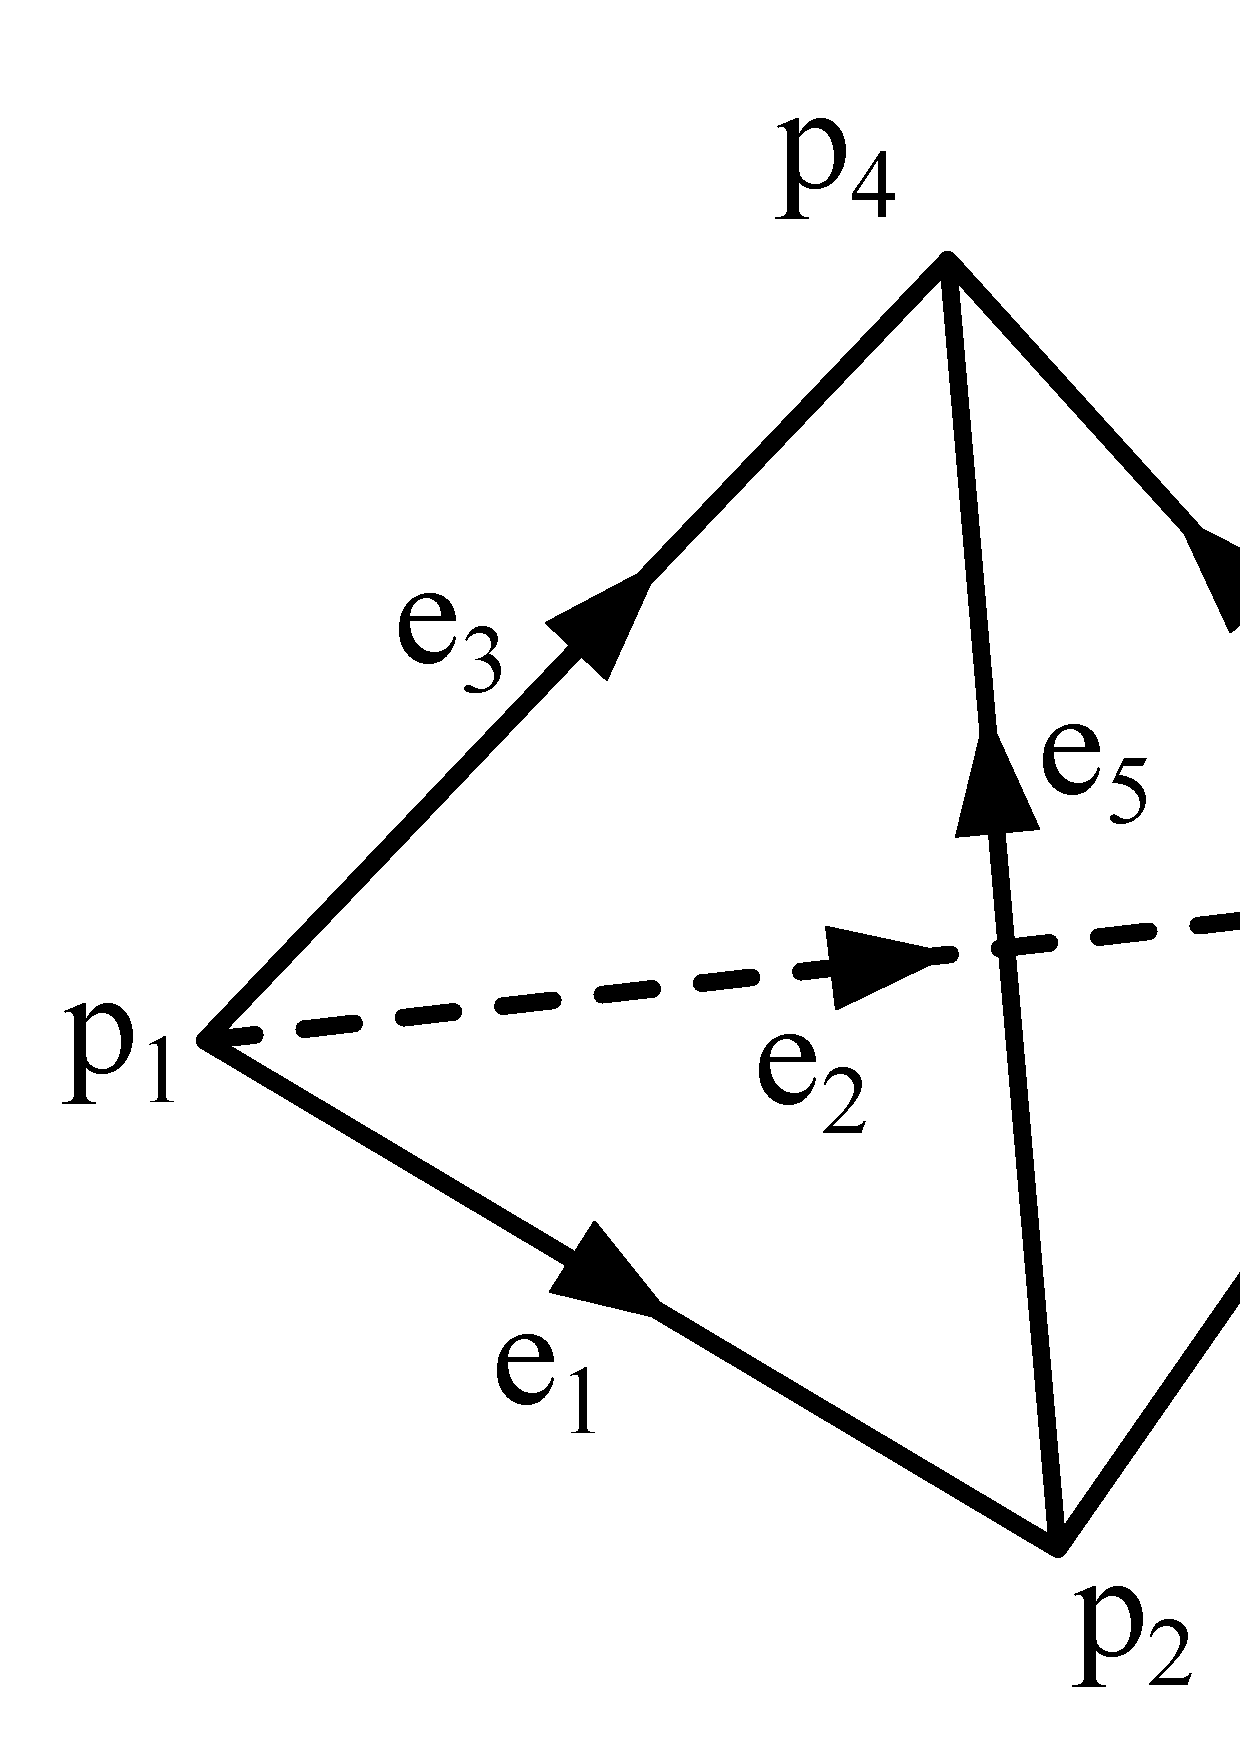
\includegraphics[scale=0.5]{tetrahedron.png}
	\caption{тетраэдральный конечный элемент}
	\label{fig:tetrahedron}
\end{figure}

Под $\mathfrak{L}$-координатами понимают функции следующего вида:
\begin{equation*}
	\mathfrak{L}_i (x, y, z) = \alpha_{i, 1} x + \alpha_{i, 2} y + \alpha_{i, 3} z + \alpha_{i, 4} , \text{~~~} i = \overline{1..4} . \label{eq:tet:L}
\end{equation*}
Коэффициенты $\alpha_{i, j}$ могут быть определены по формуле (\ref{eq:tet:D1}):
\begin{equation}
	\left[
	\begin{matrix}
		\alpha_{1, 1} & \alpha_{1, 2} & \alpha_{1, 3} & \alpha_{1, 4} \\
		\alpha_{2, 1} & \alpha_{2, 2} & \alpha_{2, 3} & \alpha_{2, 4} \\
		\alpha_{3, 1} & \alpha_{3, 2} & \alpha_{3, 3} & \alpha_{3, 4} \\
		\alpha_{4, 1} & \alpha_{4, 2} & \alpha_{4, 3} & \alpha_{4, 4} \\
	\end{matrix}
	\right] = \left[
	\begin{matrix}
		X_1 & X_2 & X_3 & X_4 \\
		Y_1 & Y_2 & Y_3 & Y_4 \\
		Z_1 & Z_2 & Z_3 & Z_4 \\
		1 & 1 & 1 & 1 \\
	\end{matrix}
	\right]^{-1} = D^{-1} . \label{eq:tet:D1}
\end{equation}

Задав $\mathfrak{L}$-координаты, можно определить на тетраэдре базисные функции. В отличие от узлового метода конечных элементов, в векторном методе конечных элементов базисные функции ассоциированы не с узлами, а с ребрами (edge), гранями (face) и объемами (volume)~\citep{nechaev, webb}. Так как будет использован полный базис первого порядка (называемый также базисом первого порядка II типа), то ограничимся рассмотрением только базисных функций, ассоциированных с ребрами.

Иерархический векторный базис Вебба первого порядка второго типа имеет вид:
\begin{equation*}
	\begin{matrix}
	\mathbf{w}_{i}^{1,\mathrm{I}} = \mathfrak{L}_k \nabla \mathfrak{L}_l - \mathfrak{L}_l \nabla \mathfrak{L}_k ; \text{~~} i = 1, ..., 6 ; \text{~~} k, l = 1, ..., 4 ; \text{~~} k < l ,\\
	\mathbf{w}_{i}^{1,\mathrm{II}} = \mathfrak{L}_k \nabla \mathfrak{L}_l + \mathfrak{L}_l \nabla \mathfrak{L}_k ; \text{~~} i = 7, ..., 12 ; \text{~~} k, l = 1, ..., 4 ; \text{~~} k < l ,
	\end{matrix}
	\label{eq:basis}
\end{equation*}
где $\mathbf{w}_{1}^{1,\mathrm{I}}, ..., \mathbf{w}_{6}^{1,\mathrm{I}}$ – базисные функции первого порядка первого типа, ассоциированные с ребрами, $\mathbf{w}_{7}^{1,\mathrm{II}}, ..., \mathbf{w}_{12}^{1,\mathrm{II}}$ – базисные функции первого порядка второго типа, ассоциированные с ребрами.

% =============================================================================

\clearpage
\addcontentsline{toc}{section}{Список литературы}
\begin{thebibliography}{10}
% 1
\bibitem{shurina} 
Шурина, Э.П. Морская геоэлектрика – задачи и перспективы / Э.П. Шурина, М.И. Эпов, А.В. Мариенко // Тезисы докладов всероссийской научно-технической конференции "Научное и техническое обеспечение исследования и освоения шельфа Северного Ледовитого океана". – 2010. – 9-13~августа. – С.~7-12.
% 2
\bibitem{gabrielsen} 
Gabrielsen, P.T. 3D CSEM for Hydrocarbon Exploration in the Barents Sea / P.T. Gabrielsen, D.V. Shantsev, S. Fanavoll // 5th Saint Petersburg International Conference \& Exhibition – Geosciences: Making the most of the Earth’s resources. – 2012. – 2-5~April. – P.~1-5.
% 3
\bibitem{berenger}
Berenger, J.P. A perfectly matched layer for the absorption of electromagnetic waves / J.P. Berenger // Jurnal of computation physics 114, 185-200, 1994
% 4
\bibitem{wiik_dehoop_ursin}
Wiik, T. A Discontinuous Galerkin Method for Modelling Marine Controlled Source Electromagnetic Data / T. Wiik, M.V. De Hoop, B. Ursin // Proceedings of the Project Review, Geo-Mathematical Imaging Group, Purdue University, West Lafayette, IN, Vol. 1 (2013) pp. 75-102.
% 5
\bibitem{epov}
Эпов, М.И. Параллельные конечноэлементные вычислительные схемы в задачах геоэлектрики / М.И. Эпов, Э.П. Шурина, Д.А. Архипов // Вычислительные технологии. – 2013. – Том~18, №2. – С.~94-112.
% 6
\bibitem{balandin} 
Баландин, М.Ю. Векторный метод конечных элементов : Учеб. пособие / М.Ю. Баландин, Э.П. Шурина. – Новосибирск : Изд-во НГТУ, 2001. – 69~с.
% 7
\bibitem{webb}
Webb, J.P. Hierarchal Vector Basis Functions of Arbitrary Order for Triangular and Tetrahedral Finite Elements / J.P. Webb // IEEE transactions on antennas and propagation. – 1999. – Vol.~47. – P.~1244-1253.
% 8
\bibitem{nechaev}
Nechaev, O.V. Multilevel iterative solver for the edge fem solution of the 3D Maxwell equation / O.V. Nechaev, E.P Shurina, M.A. Botchev // Computers and Mathematics with Applications. – 2008. – №55. – P.~2346-2362.
% 9
\bibitem{soloveychick}
Соловейчик, Ю.Г. Метод конечных элементов для решения скалярных и векторных задач : учеб. пособие / Ю.Г. Соловейчик, М.Э. Рояк, М.Г. Персова. – Новосибирск : Изд-во НГТУ, 2007. – 896~с.
\end{thebibliography}

% =============================================================================


\end{document}
